% !TEX program = xelatex
\documentclass[]{article}
\usepackage{commons/course}

\begin{document}
\printheader

در این تمرین می‌خواهیم که به کمک کتابخانه‌ی
\lr{TrueTime} و برنامه \lr{Matlab}
یکی از مثال‌های آن را شبیه سازی کنیم.

\section*{نسخه 5.1 TrueTime}
همان طور که در تمرین گفته شده بود من می‌خواستم که در ابتدا مثال
\lr{Mobile Motes}
را در متلب اجرا کنم. این مثال تنها در نسخه‌ی
\lr{1.5}
وجود دارد و در نسخه‌ی آخر آن (۲) وجود ندارد.
به همین جهت من نسخه‌ی
\lr{1.5}
را از
\link{http://archive.control.lth.se/media/Research/Tools/TrueTime/truetime-1.5.zip}{این لینک}
دانلود کردم. سپس طبق فایل
\lr{PDF}
درون آن در ابتدا باید خط‌های زیر را در فایل
\verb|Documents/MATLAB/startup.m|
قرار می‌دادم:
\begin{latin}
\begin{lstlisting}
addpath([getenv('TTKERNEL')]);
init_truetime;
\end{lstlisting}
\end{latin}
همچنین باید به
\lr{environemnt variable}های
سیستم‌عامل مقدار
\verb|TTKERNEL|
را برابر مسیر نسخه‌ی از حالت فشرده خارج شده و فولدر
\lr{kernel}
قرار دهیم.
من آخرین نسخه‌ی متلب یعنی
\lr{2023b}
را نصب کرده بودم و با همین نسخه در ابتدا متلب را باز کردم و به فولدر
\lr{motes}
در فولدر
\lr{examples}
رفتم. با توجه به فایل
\lr{readme}
در ابتدا در
\lr{command line}
خود متلب فایل
\lr{init}
را اجرا کردم و سپس بر روی فایل
\verb|motes.mdl|
دو بار کلیک کردم که باز شود در نهایت نیز از بالای صفحه بر روی دکمه‌ی
\lr{Run}
کلیک کردم. اما در کنسول اروری مثل ارور شکل
\ref{fig:1.5-error-run}
آمد:
\begin{figure}[H]
    \centering
    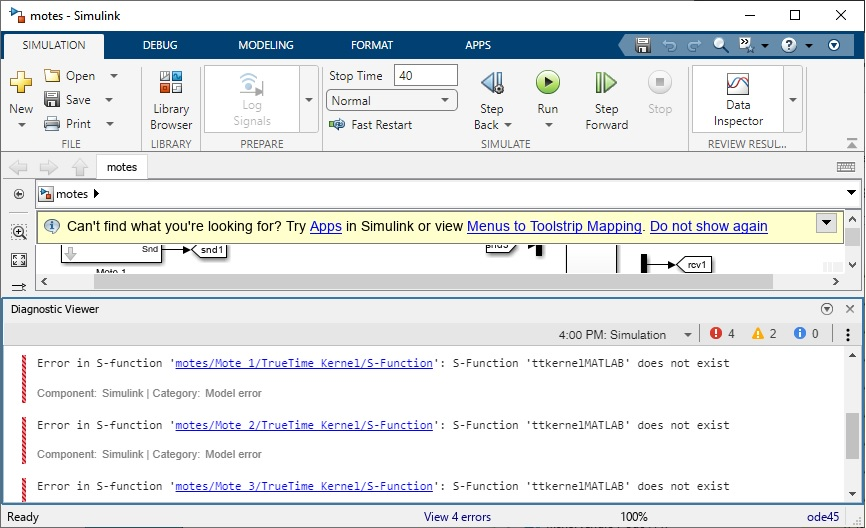
\includegraphics[scale=0.6]{pics/1.5-error.jpg}
    \caption{ارور خوردن در اجرای مثال \lr{Mobile Motes}}
    \label{fig:1.5-error-run}
\end{figure}
با کمی تحقیق در اینترنت متوجه شدم که مشکل این ارور است است که کتابخانه‌ای برای نسخه‌ پردازنده شما کامپایل نشده است.
به همین منظور از آنجا که خودم
\lr{visual studio}
را نصب داشتم سعی کردم که کتابخانه را یک بار از اول کامپایل بکنم. اما باز هم به مشکلی خوردم که کتابخانه
از یک تابع قدیمی استفاده می‌کرد که در نسخه‌های جدیدتر متلب وجود ندارد. عکس این ارور در شکل
\ref{fig:1.5-error-compile}
آمده است:
\begin{figure}[H]
    \centering
    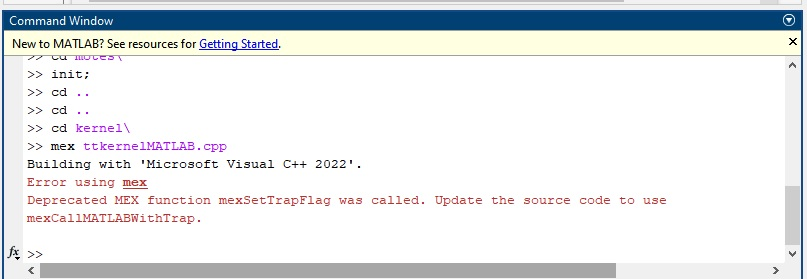
\includegraphics[scale=0.6]{pics/1.5-error-compile.jpg}
    \caption{ارور خوردن در کامپیال کردن مجدد \lr{TrueTime}}
    \label{fig:1.5-error-compile}
\end{figure}
اما با همه‌ی این مشکلات حداقل پنجره‌ی
\lr{figure}
باز میشد! (ولی چیزی حرکت نمی‌کرد)
\begin{figure}[H]
    \centering
    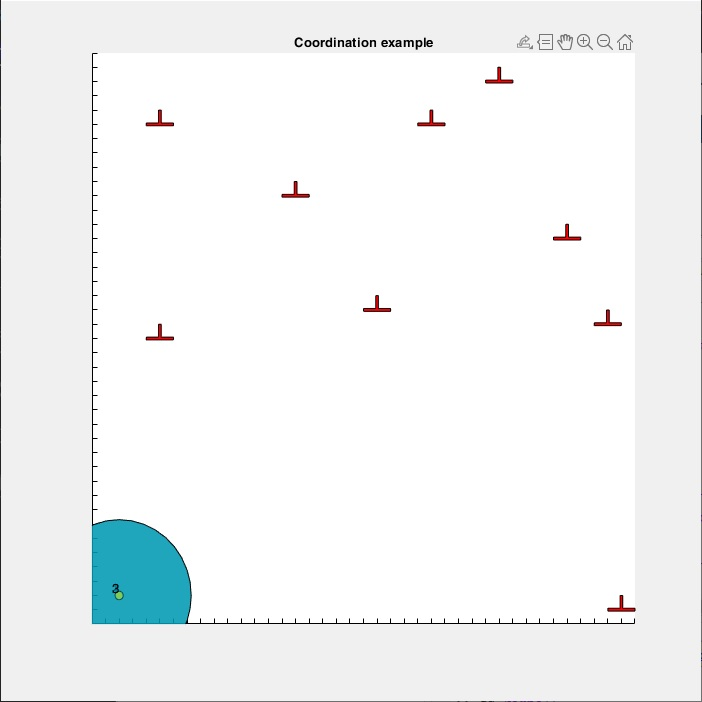
\includegraphics[scale=0.6]{pics/motes.jpg}
    \caption{باز شدن پنجره figure}
\end{figure}
به همین منظور من سعی کردم که نسخه‌ی ۲ کتابخانه
\lr{TrueTime}
را استفاده کنم.
\section*{نسخه 2 TrueTime}
در ابتدا من نسخه‌ی ۲ این کتابخانه را از
\link{http://archive.control.lth.se/media/Research/Tools/TrueTime/truetime-2.0.zip}{این لینک}
دانلود کردم. سپس آنرا در جایی از حالت فشرده سازی شده خارج کردم و در برنامه‌ی
\lr{Matlab}
به کمک
\verb|cd|
به آن فولدر رفتم و فایل
\verb|init_truetime.m|
را در
\lr{command line}
اجرا کردم.

متاسفانه در این نسخه از کتابخانه مثال
\lr{Mobile Motes}
وجود ندارد. من حتی سعی کردم که مثال را از ورژن
\lr{1.5}
به این نسخه بیاورم ولی از آنجا که
\lr{API}
کتابخانه عوض شده بود امکان اجرای آن را نداشتم.
\begin{figure}[H]
    \centering
    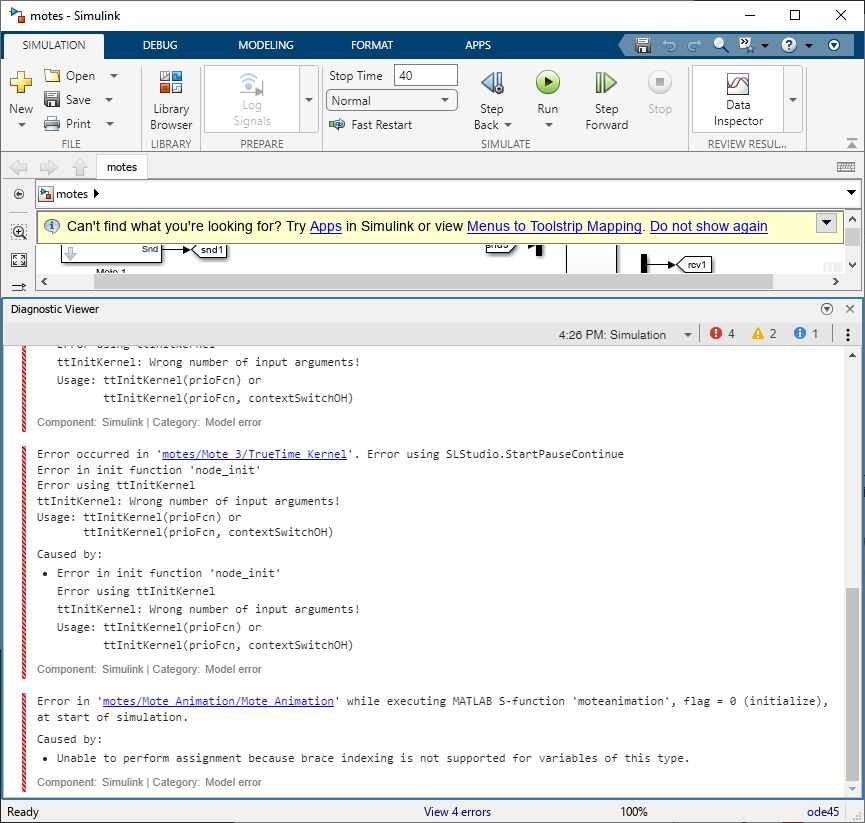
\includegraphics[scale=0.6]{pics/2-error.jpg}
    \caption{خطای اجرای \lr{Mobile Motes} بر روی نسخه‌ی ۲ TrueTime}
\end{figure}
اما من مثال
\lr{soccer}
را اجرا کردم. در این مثال صرفا کافی بود که فایل
\verb|soccer.slx|
را باز کنم و در پنجره باز شده بر روی دکمه‌ی
\lr{run}
کلیک کنم.
\begin{figure}[H]
    \centering
    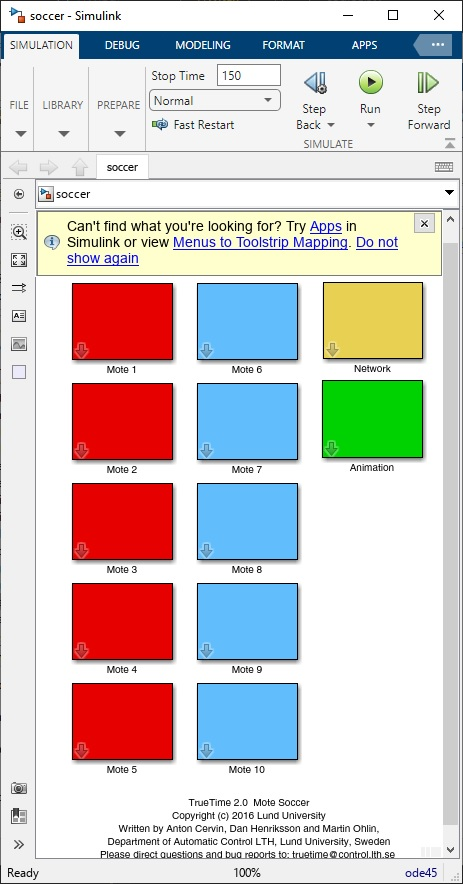
\includegraphics[scale=0.6]{pics/soccer.jpg}
    \caption{پنجره‌ی فایل \lr{soccer.slx}}
\end{figure}
\begin{figure}[H]
    \centering
    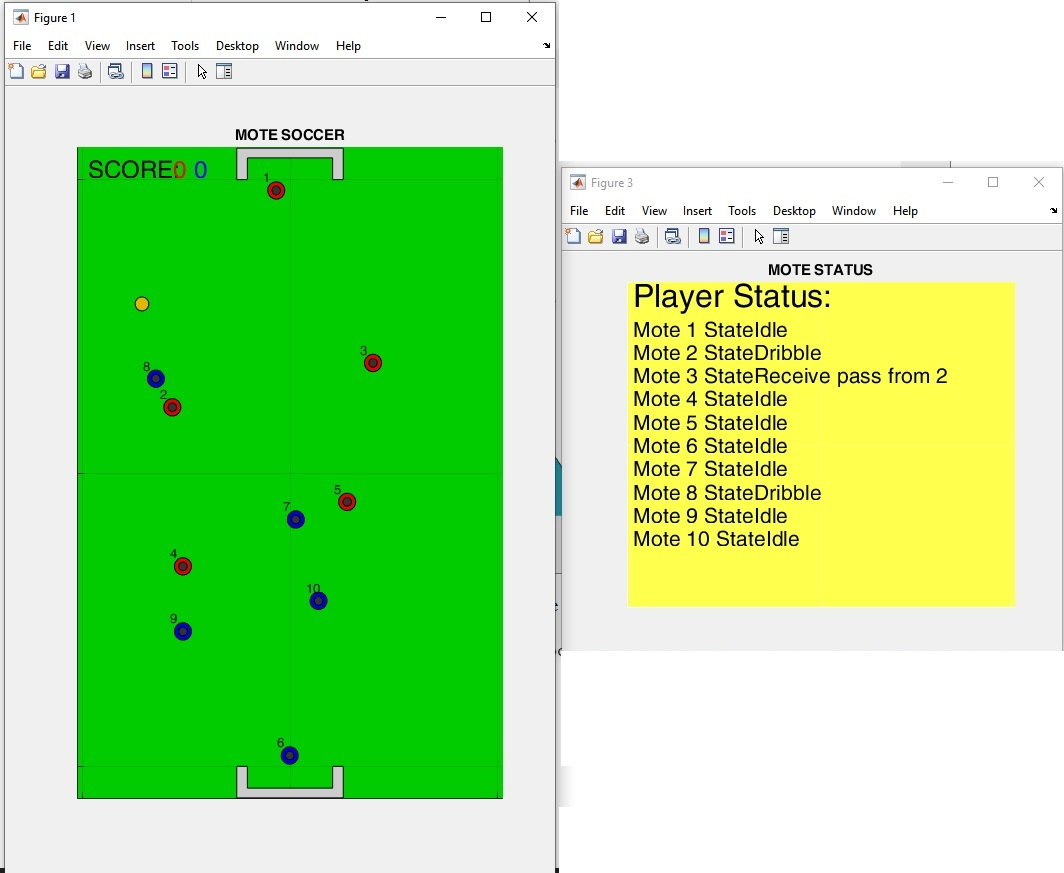
\includegraphics[scale=0.5]{pics/soccer-run.jpg}
    \caption{اجرای بازی}
\end{figure}
همان طور که مشاهده می‌کنید بازی با موفقیت اجرا شد.
\end{document}
